\documentclass[brudnopis]{xmgr}
% Jeśli nowe rozdziały mają się zaczynać na stronach
% nieparzystych:
%\documentclass[openright]{xmgr}

%\defaultfontfeatures{Scale=MatchLowercase}
%\setmainfont[Numbers=OldStyle,Ligatures=TeX]{Minion Pro}
%\setsansfont[Numbers=OldStyle,Ligatures=TeX]{Myriad Pro}
% for fontspec version < 2.0
\setmainfont[Numbers=OldStyle,Mapping=tex-text]{Minion Pro}
\setsansfont[Numbers=OldStyle,Mapping=tex-text]{Myriad Pro}
%\setmonofont[Scale=0.75]{Monaco}

% Opcjonalnie identyfikator dokumentu
% drukowany tylko z włączoną opcją 'brudnopis':
\wersja   {wersja wstępna [\ymdtoday]}

\author   {Marcin Dawidowski}
\nralbumu {231010}
\email    {marcin.dawidowskipl@gmail.com}

\title    {Let’s Bid It – portal aukcyjny}
\date     {2017}
\miejsce  {Gdańsk}

\opiekun  {dr Włodzimierz Bzyl}

% dodatkowe polecenia
%\renewcommand{\filename}[1]{\texttt{#1}}
%\definecolor{stress}{cmyk}{0,1,0.13,0} % RubineRed
%\definecolor{topic}{cmyk}{0.98,0.13,0,0.43} % MidnightBlue

\begin{document}

% streszczenie
\begin{abstract}
  W pracy przedstawiono wersję beta aplikacji webowej „Let's Bid It” do tworzenia i publikowania aukcji.
  
  W aplikacji zaimplementowano kategoryzację aukcji, wyszukiwanie, a także tworzenie kategorii w hierarchii.

  Zaprojektwano widok strony głównej, który wyświetla losowe aukcje znajdujące się w portalu oraz panele administracyjny i użytkownika, które są widoczne po zalogowaniu się na konkretny typ konta. Każda z aukcji wyświetlana jest w kolejności rosnącej według czasu zakończenia.

  Do tworzenia aplikacji wykorzystano Ruby on Rails, a także Twitter Bootstrap do implementacji widoków. Użyto również gemu CKEditor pozwalający umieścić na stronie zaawansowany edytor tekstowy. Do stworzenia drzewa kategorii użyto gemu Acts as tree.

\end{abstract}

% słowa kluczowe
\keywords{Ruby on Rails, gem, heroku, auction, online shopping, bid}

% tytuł i spis treści
\maketitle

% wstęp
\introduction

Chęć stworzenia czegoś od podstaw oraz własne doświadczenie w korzystaniu z portali aukcyjnych sprawiło, że dla mnie jako programisty stworzenie takiej aplikacji, byłoby niezwykle satysfakcjonujące i pozwoliłoby rozwinąć umiejętności. Ponadto stworzenie takiego portalu może ułatwić mi w przyszłości implementacje różnego rodzaju sklepów internetowych i innych serwisów związanych z handlem przez Internet.


\chapter{Wstęp}

W dzisiejszych czasach bardzo wiele osób korzysta z portali aukcyjnych. 
Dzieję się tak przede wszystkim dlatego, że pomagają one zdecydowanie
zaoszczędzić czas, a także w dużej mierze pozwalają oszczędzić 
pieniądze, dzięki konkurencyjnym cenom oraz szerokiemu wahlarzowi dostępnego
towaru. Powstało już wiele stron, które pozwalają nam dokonywać zakupów w 
domowym zaciszu, jednak każda z nich posiada pewne cechy, które odróżniają
je od konkurencji. Tworząc tą aplikację miałem na celu wyłapać jak najwięcej 
tych cech i umieścić je w moim projekcie, który będzie je łączył.


\section{Porównanie z dostępnymi rozwiązaniami}

\subsection{Allegro} 

Jest to największa, a także najpopularniejsza platforma transakcyjna on-line w Polsce, oferująca setki produktów w niezwykle konkurencyjnych cenach. Serwis udostępnia możliwość zakupu natychmiastowego, licytacji, a także wystawiania ogłoszeń. Typ danej aukcji, zależy tylko i wyłącznie od jej właściciela.

Jeśli chodzi o wystawianie aukcji, to proces wygląda podobnie do Let's Bid It. Tak jak w mojej aplikacji użytkownik może skorzystać z zaawansowanego edytora tekstowego, dodaje zdjęcia i przyporządkowuje ją do konkretnej kategorii. Główną różnicą jest fakt, że Allegro pozwala na wystawienie przedmiotu z opcją "Kup Teraz", lub też jako ogłoszenie.

\subsection{OLX}  

Serwis ten jest jednym z najpopularniejszych portali ogłoszeniowych na świecie. Użytkownicy
mogą udostępniać lokalne ogłoszenia dotyczące sprzedaży oraz usług. Główną różnicą pomiędzy OLX, a Let's Bid It jest fakt,
że wymieniony wyżej portal nie udostępnia funkcji licytacji towaru, dlatego też nie ma możliwości, by osoba wystawiająca ogłoszenie mogła sprzedać swój towar drożej niż w ogłoszeniu. Ponadto stworzony przeze mnie portal aukcyjny dzięki zaawansowanemu edytorowi tekstowemu pozwala stworzyć użytkownikom dużo bardziej oryginalne opisy, co nie jest możliwe przy korzystaniu z OLX.

\section{Możliwości zastosowania praktycznego}
Głównym założeniem serwisu Let's Bid It jest przede wszystkim portal aukcyjny i jest to główna możliwość zastosowania napisanej przeze mnie aplikacji w praktyce. Poza tym portal ten użyty może zostać również do innych celów.

\begin{itemize}

\item Portal ogłoszeniowy - jest jedna z możliwości wykorzystania Let's Bid It w praktyce. Potrzeby takiej aplikacji zaspokajają praktycznie wszystkie wdrożone w mojej aplikacji funkcjonalności, takie jak kategoryzacja, a także prosta obsługa dodanych ogłoszeń. Ponadto użytkownik takiego  serwisu będzie miał do dyspozycji bardzo prosty interfejs ułatwiający poruszanie się po stronie, a także zaawansowany edytor, który pozwoli na to, by jego ogłoszenie wyglądało wyjątkowo.

\item Sklep internetowy - jest to kolejna możliwa opcją zastosowania mojej aplikacji w praktyce, co można osiągnąć przy niedużym nakładzie pracy. Tak jak przy portalu ogłoszeniowym, dostępne są przede wszystkim kategoryzacja, a także obsługa dodawanych aukcji oraz zaawansowane narzędzia do zarządzania wyglądem aukcji.

\end{itemize}

\chapter{Projekt i analiza}

\section{Diagram ERD}

\begin{figure}[!tbh]
\centering
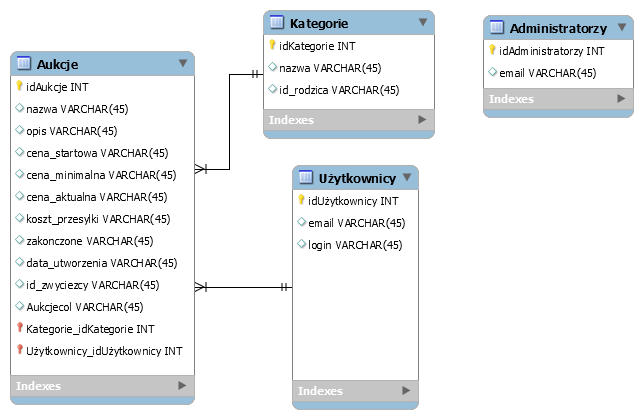
\includegraphics[width=.8\linewidth]{erd}
\caption{Diagram związków encji\label{RYS.1}}
\source{Opracowanie własne}
\end{figure}

\section{Aktorzy i przypadki użycia}

\section{Diagram klas}

\chapter{Implementacja}
W celu stworzenia aplikacji, która ma w odpowiedni sposób realizować postawione przed nią
założenia, potrzebne są odpowiednio dobrane technologie oraz narzędzia, dzięki którym uda się 
spełnić postawione przed nią wymagania. Dobór odpowiedniej technologii, a także frameworków 
jest kluczowy do skutecznej implementacji aplikacji. Poniżej omówię wybrane przeze mnie narzędzia oraz to co udało się, a także nie udało się zrealizować.

\section{Realizacja projektu}

Aplikacja Let's Bid It jest wersją beta portalu aukcyjnego, dlatego też nie posiada jeszcze wszystkich funkcjonalności, które pozwoliłyby w pełni wykorzystać potencjał serwisu. Poniżej przedstawię funkcjonalności, które udało się wdrożyć, a także te, których nie udało się zaimplementować.

\subsection{Założenia zrealizowane}

Na dzień dzisiejszy udało się zrealizować przede wszystkim obsługę aukcji, to znaczy, każdy zalogowany użytkownik może stworzyć
własną aukcję, licytować aukcje innych użytkowników, wyszukiwać aukcje, edytować je, lub usuwać. W celu lepszego wyszukiwania aukcji wdrożona została także kategoryzacja aukcji przy pomocy gemu Act as tree.

Kolejną rzeczą jest wdrożenie zaawansowanego edytora tekstowego CKEditor, dzięki któremu dodając aukcję, użytkownik może swobodnie manipulować opisem swojej aukcji.

Ważnym elementem Let's Bid It jest również grafika dołączana do każdej aukcji. W związku z tym, że aplikacja znajduje się na platformie Heroku, głównym problemem było przetrzymywanie plików graficznych, które na Heroku usuwane są automatycznie. Rozwiązaniem tego problemu okazało się skorzystanie z serwisu Cloudinary, który pozwala bezpłatnie przechowywać pliki w chmurze, a co najważniejsze, możliwe jest skonfigurowanie go tak, by współpracował z aplikacją napisaną w Ruby on Rails, w czym pomocny okazał się gem cloudinary.

Udało się również zaimplementować zabezpieczenie reCaptcha, pozwalające na dopuszczenie do przesyłu danych wypełnionych tylko i wyłącznie przez prawdziwego użytkownika.

\subsection{Założenia niezrealizowane}

Najważniejszą rzeczą, której nie udało się zrealizować jest wdrożenie systemu mającego na celu symulacje płatności internetowych, a także zaawansowana wyszukiwarka opierająca się na silniku Elasticsearch.

\section{Ruby on Rails}
Do stworzenia projektu wykorzystana została technologia Ruby on Rails bazująca na języku Ruby.
W aplikacji wykorzystano Ruby w wersji 2.3, a także framework Rails w wersji 5.0.1. Całość stworzona
została przy pomocy architektury MVC (ang. Model-View-Controller).

\section{Twitter Bootstrap}
Widoki utworzone zostały przy pomocy frameworka Twitter Bootstrap, który pozwala na proste tworzenie
graficznego interfejsu stron internetowych z wykorzystaniem gotowych rozwiązań bazujących na językach
HTML i CSS. Główną zaletą tego frameworka jest responsywność, czyli zapewnienie dobrego wyświetlania
stron WWW na różnego typu urządzeniach. 

\section{Pozostałe rozwiązania użyte przy realizacji projektu}

CKEditor - jest to wizualny edytor tekstowy języka HTML, który umożliwia użytkownikowi na wybranie między innymi konkretnej 
czcionki, jej rozmiaru, koloru liter, czy też ich stylu. Poza tym użytkownik może również ustawić wyrównanie tekstu,
a także możliwe jest wstawienie listy, tabeli, odnośników, a także obrazów.

Act as tree - gem ten wykorzystany został w celu stworzenia drzewa kategorii, które ułatwia w sposób zdecydowany nawigację
po stronie, a także sprawia, że dane na stronie są uporządkowane. Sama implementacja przebiega w środowisku
technologii Ruby on Rails, więc nie wymaga bezpośredniej instalacji.

reCaptcha - zabezpieczenie dzięki któremu możliwość wysyłania danych będą mieli jedynie sprawdzeni użytkonicy.

% zakończenie
\summary

% załączniki (opcjonalnie):
\appendix
\chapter{Tytuł załącznika jeden}

Treść załącznika jeden.

\chapter{Tytuł załącznika dwa}

Treść załącznika dwa.

% literatura (obowiązkowo):
\bibliographystyle{unsrt}
\bibliography{xml}

% spis tabel (jeżeli jest potrzebny):
\listoftables

% spis rysunków (jeżeli jest potrzebny):
\listoffigures

\oswiadczenie

\end{document}
